\documentclass[class=article, crop=false]{standalone}
\usepackage[subpreambles=true]{standalone}
\usepackage{import}
\usepackage[T1]{fontenc}
\usepackage[utf8]{inputenc}
\usepackage[english, danish]{babel}
\usepackage{graphicx,wrapfig,lipsum}

\begin{document}
DKD’en er det mest omfattende diagram, og man vil her kunne se både klassevariabler og metoder for de forskellige klasser i programmet. Programmet bliver startet af en Main (ikke vist på DKD’en) som står for at oprette klassen GameController, der holder styr på at resten af programmet bliver kørt ordentligt. I nogle af klasserne skal man bruge input fra brugeren, her vil man kommunikerer via GUIBoundary, der står for at oversætte vores program med den givne GUI - da vi ikke har mulighed for at rette i den. \par
Man kan også nævne brugen af generalisering på både ChanceCards og Square, der også bliver videre generaliseret via PropertySquare (kan ses på en nedstående figur~\ref{fig:DKD_udklip}). Dette gør at man via abstrakte metoder kan slippe for at duplikerer kode i sub-klasserne. Dette er også blevet brugt i en ikke vist klasse (da den kun bliver brugt til tests), MockGUI, der extender vores GUIBoundary. Den er essentiel for testene kan blive kørt, da programmet ellers venter på input fra brugeren.

\begin{figure}[H]
    \centering
    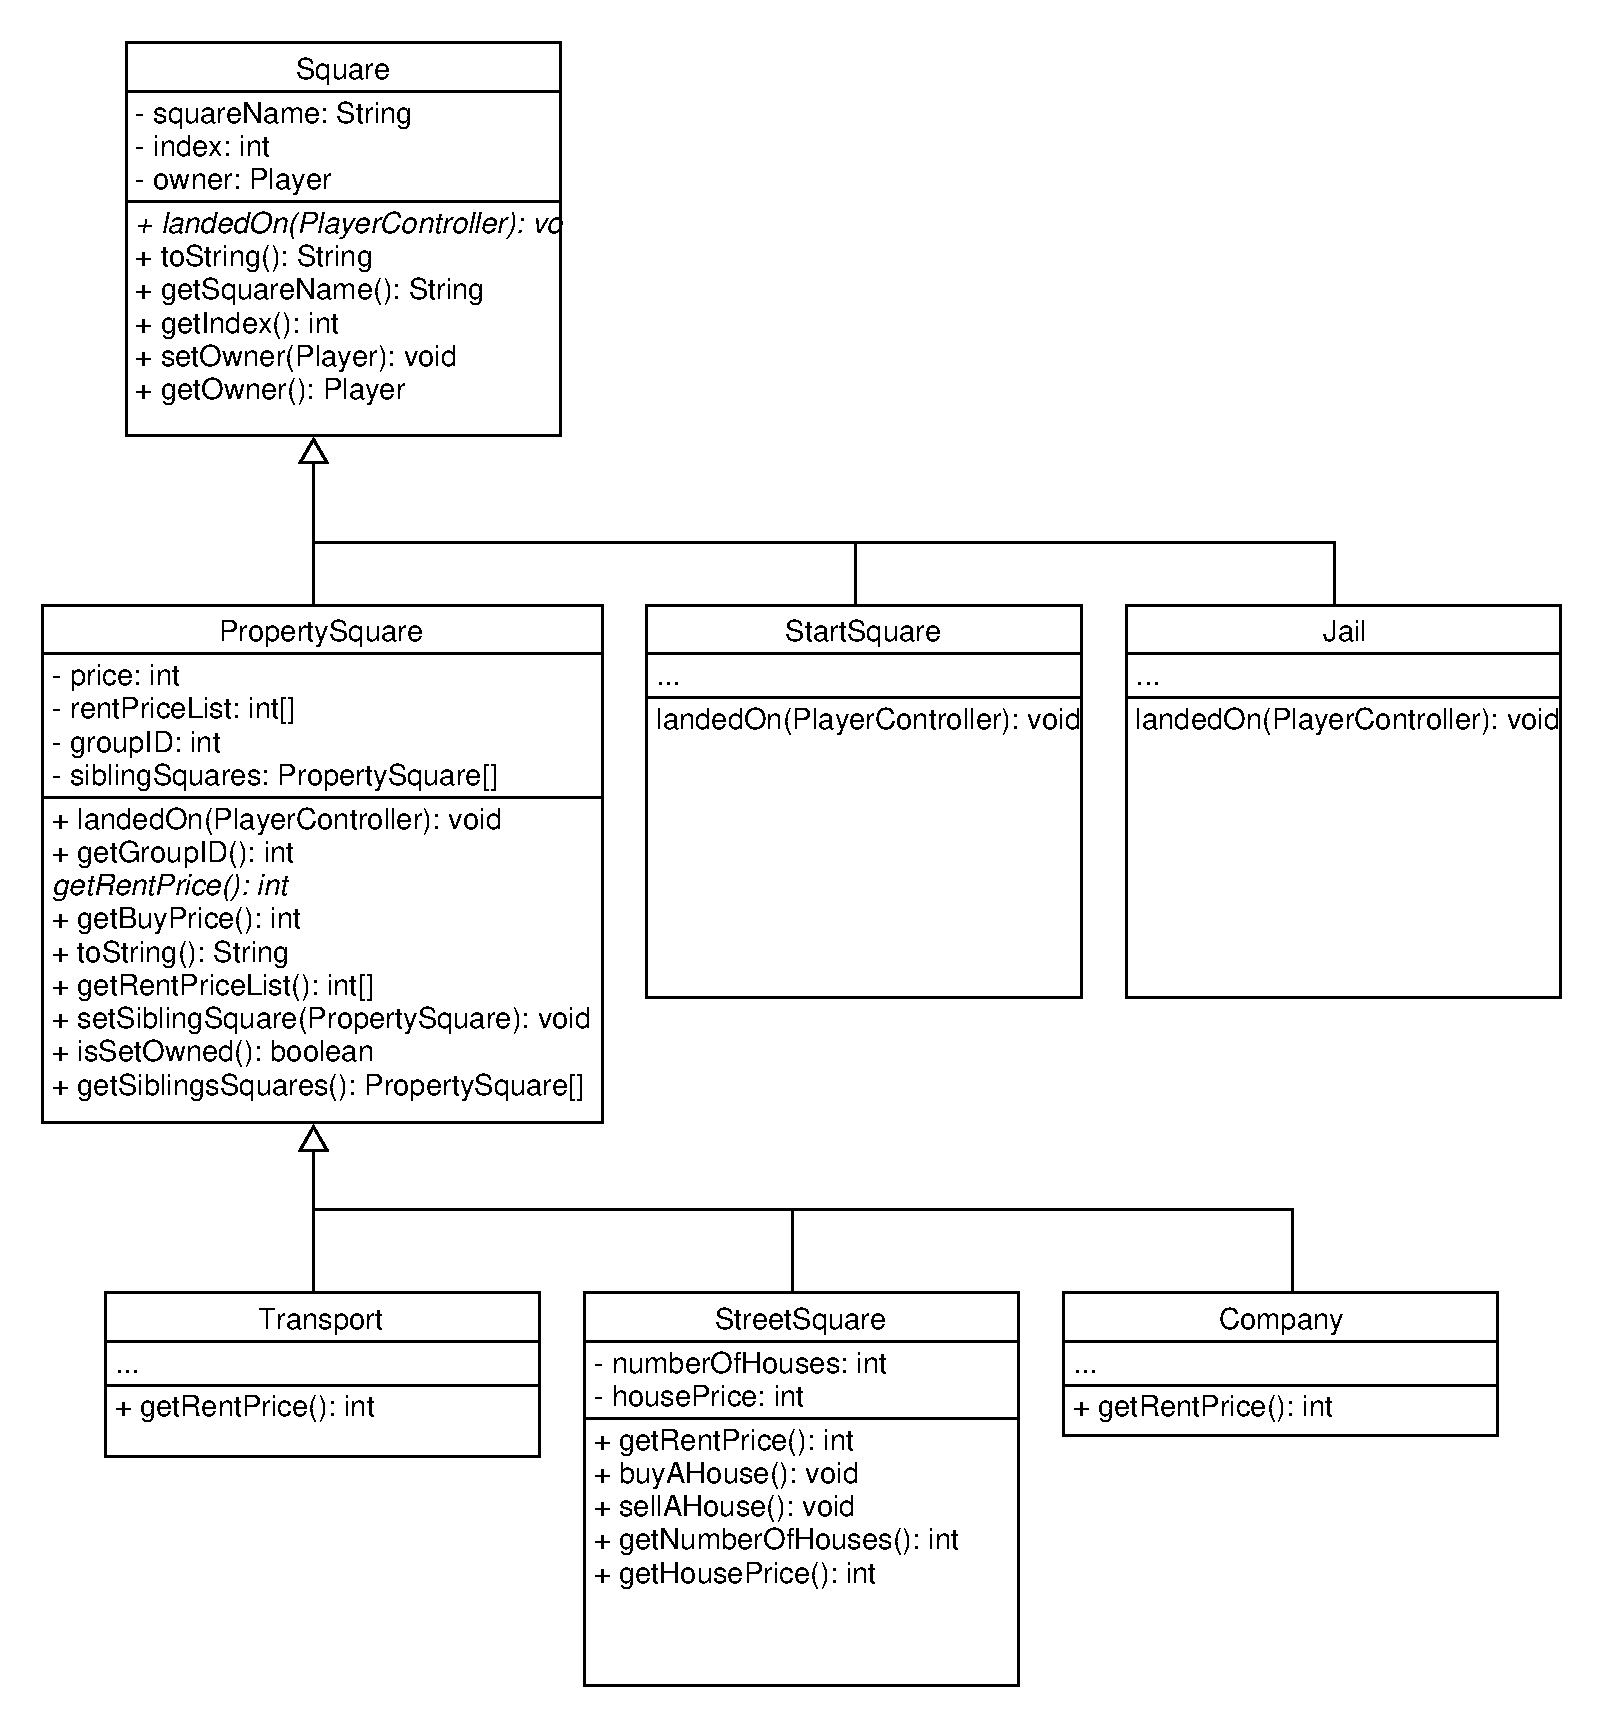
\includegraphics[scale = 0.5]{diagrams/DKD_udklip.pdf}
    \caption{Udklip fra desingklassediagrammet}\label{fig:DKD_udklip}
\end{figure}

\newpage
    \begin{figure}[H]
        \centering
        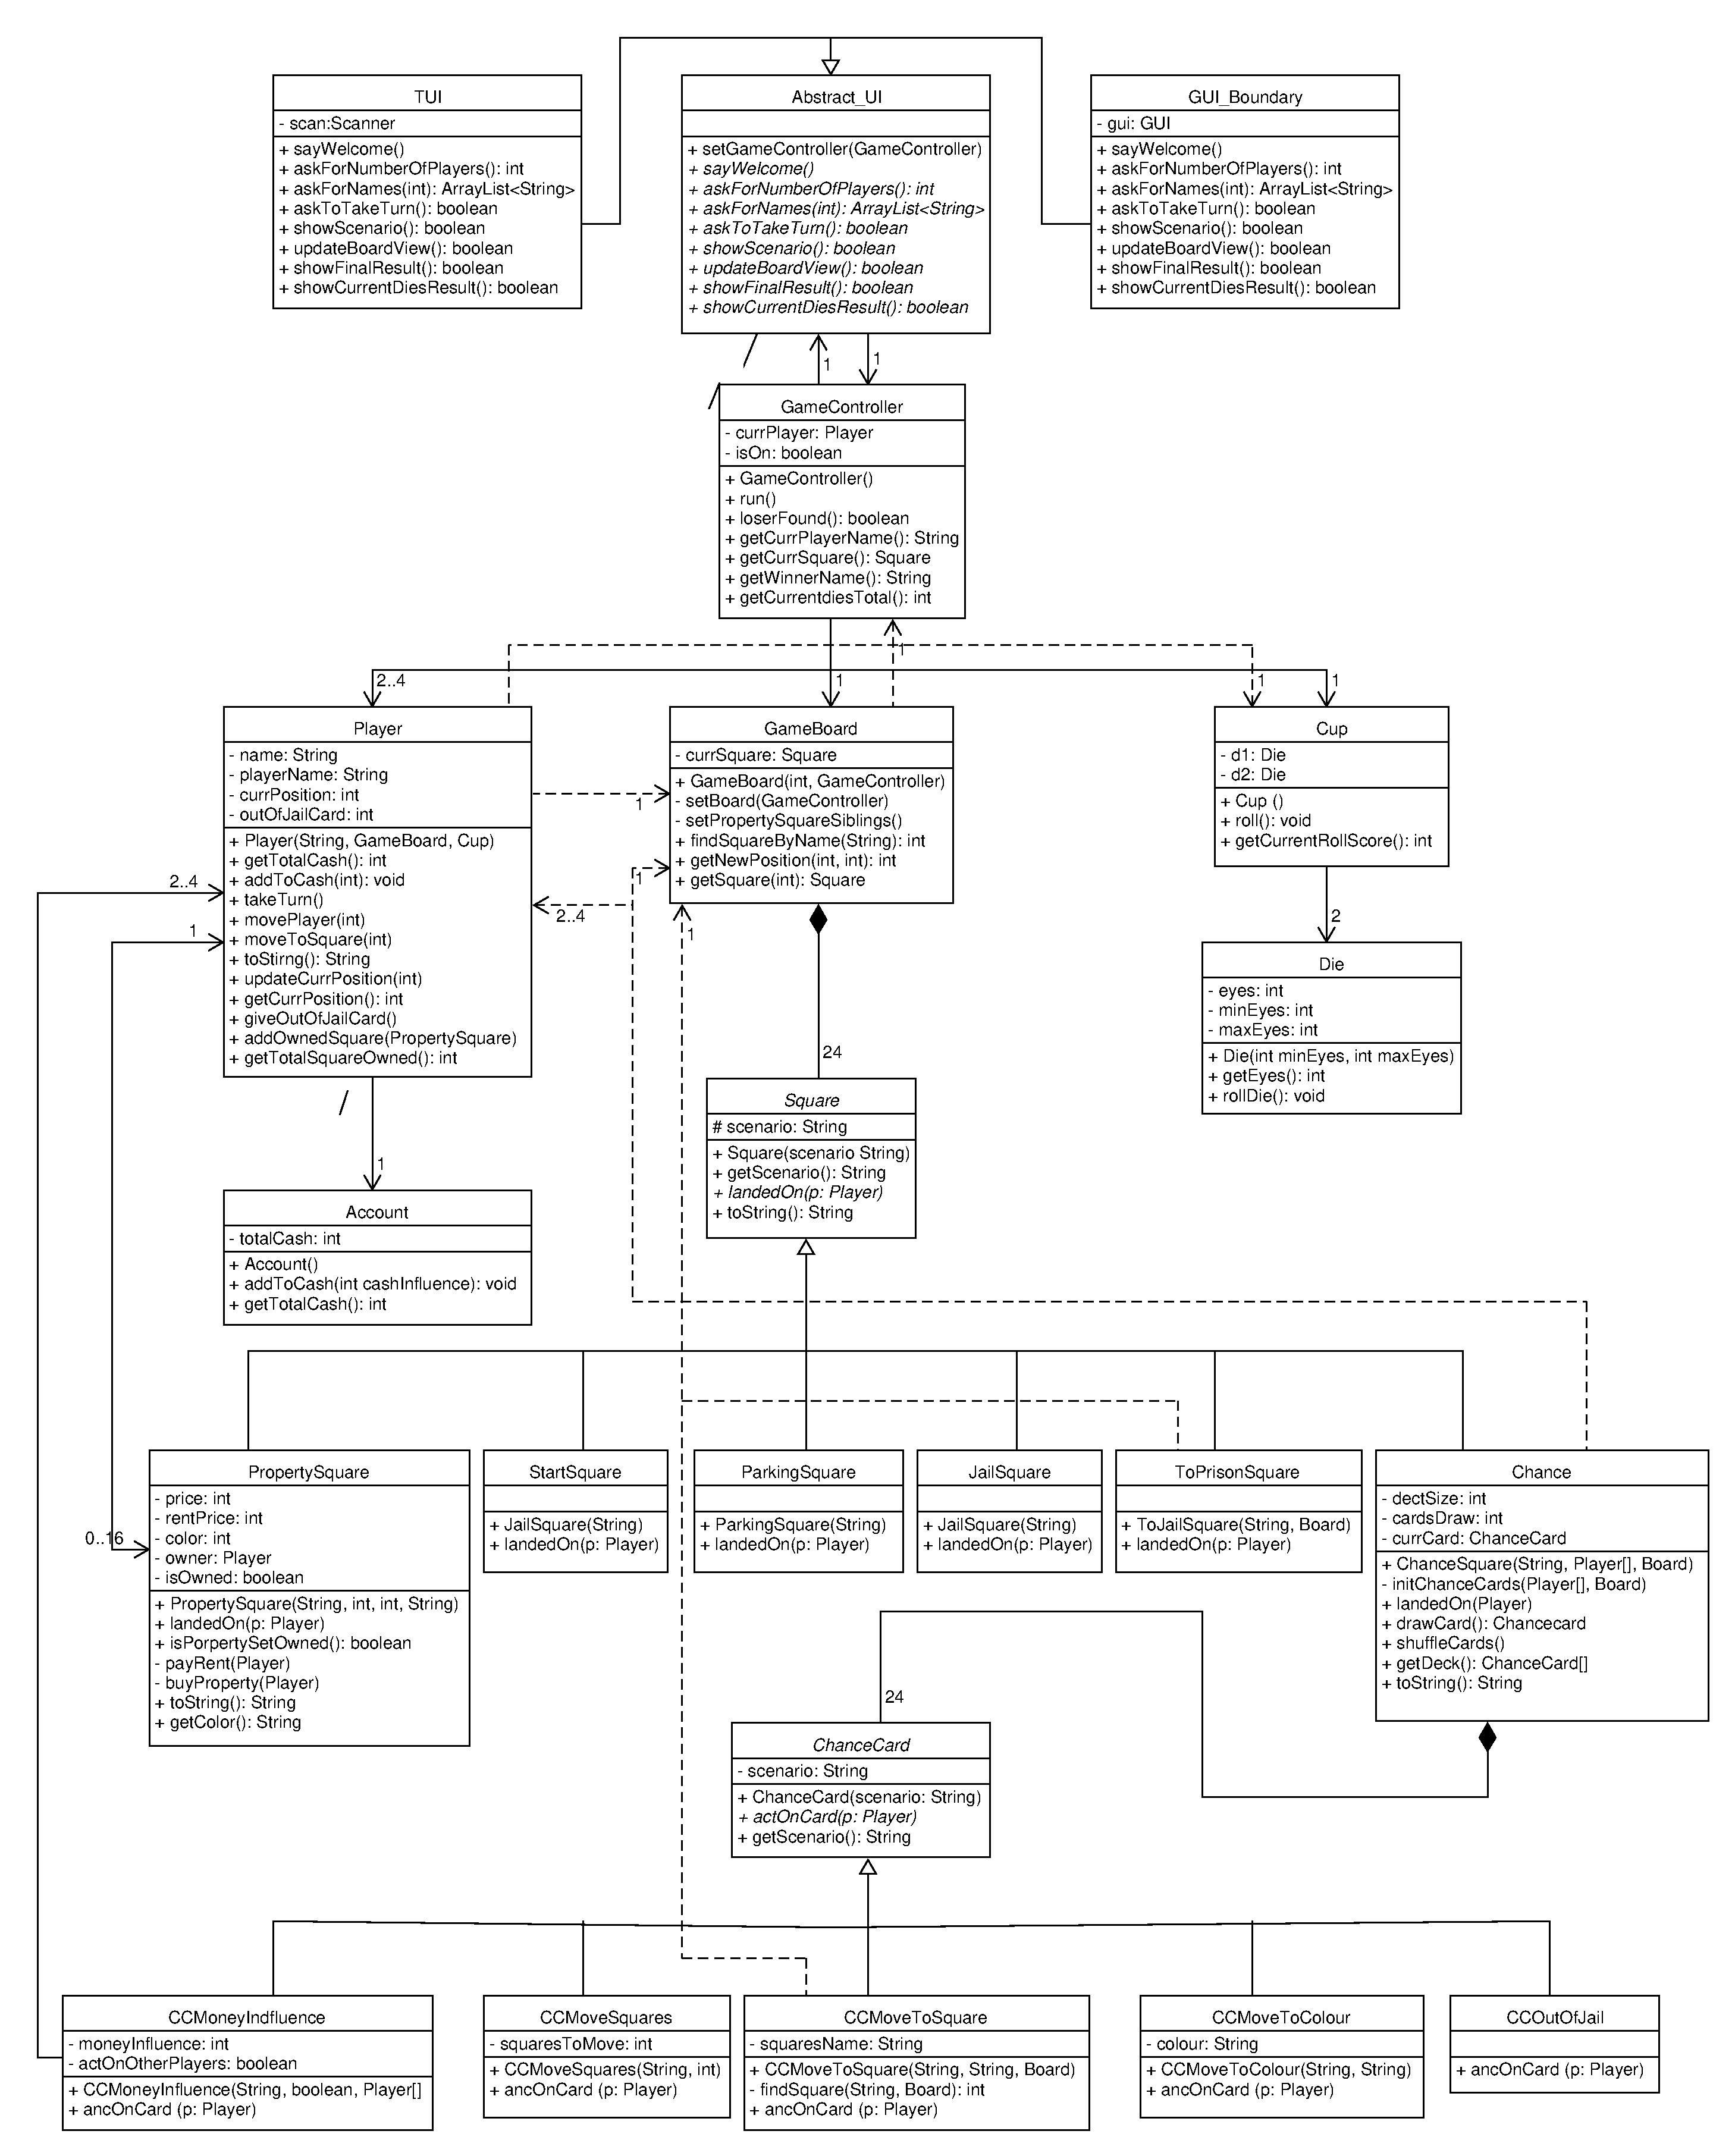
\includegraphics[scale = 0.2]{diagrams/DKD.pdf}
        \caption{Desingklassediagram over hele systemet}\label{fig:DKD}
    \end{figure}
\end{document}